\section{Raw Data Extraction}
\label{section:data_extraction}

The first task is the extraction of user data from the Ask.fm website. Before discussing the user data it is important to understand the criteria used to select which users data will be scraped. The most significant criteria is that the predominant language used is English. It would have been outside the scope of this research to consider languages other than English. The second criteria was that the user had at least one thousand, but no more than five thousand, question and answers. There were no other restrictions placed on which users data were eligible for selection.

Each users entire dataset of questions and answers is available from a single URL in the format \url{http://ask.fm/user_id} where the user id is a unique identifier for each account on the website. It is worth looking again at the layout of the individual questions as they are presented on the screen before then looking under the covers at the structure of the underlying HTML.

Figure \ref{fig:chapter4:sample_question} shows a sample question and answer from the Ask.fm site and the parts numbered one through six can be identified as follows:

\begin{enumerate}
	\item  This is the question that was asked.
	\item  The answer given to the question.
	\item  A time indication of when the question was answered.
	\item  The identity of the user that asked the question. Nothing is shown when the question is asked anonymously.
	\item  The report flag to report the question and or answer.
	\item  The number of likes that this question and answer has received. The heart icon can be used by a user of the site to show that they like this question and answer.
\end{enumerate}

\begin{figure}[htbp]
	\centering
	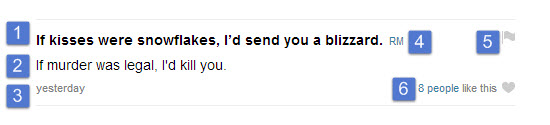
\includegraphics[width=0.85\textwidth]{Figures/Chapter4/sample_question.jpg}
	\caption[Sample question and answer]{Sample question and answer from ask.fm showing the question, the answer, when the question was answered, the user that asked the question, the report question flag and the number of likes that this question and answer has.}
	\label{fig:chapter4:sample_question}
\end{figure}

All questions and answers belonging to a single user can be displayed on a single web page. Initially, only the first 25 are displayed but a "View More" button makes it extremely easy to access all of a users questions and answers without the need for complicated scraping rules. Once all the questions and answers belonging to a user are displayed it is just a simple matter of saving the web page to a HTML file on disk.

Once the criteria to select potential users and the method to extract the users raw data was determined the final action was to download a suitably sized dataset. Having considered the downloading process in advance the goals were to obtain at least 100,000 questions and answers and to try and spread the distribution of the users as much as possible across the globe.  It was estimated that there would be an average of approximately 2,000 questions and answers per user account. To meet the first goal at least fifty accounts would be downloaded. To achieve the second goal the data was downloaded in three separate sessions each spaced over a twenty-four hour period. The first set was downloaded early in the morning local time at around 09:00. The second set was download in the early evening around 16:00. The final set was downloaded at 23:00 at night. The final action was to determine which users data to download. 

The stream page displays the most recently submitted questions and answers so this page was used to identify potential user accounts. Starting at the top, and working through all twenty five questions on the page, each users account was examined to determine if it met the criteria for selection. If it did then the users complete set of questions and answers were download. If the criteria were not met then the next users questions were examined until all questions on the stream had been reviewed. When there were no further users questions to be examined the stream was refreshed. The process was repeated until a proportional amount of user data had been downloaded at each time slot.

Upon completion, data from 57 accounts had been downloaded yielding 109,312 questions and answers. A cursory examination of the users showed that there was representation from North America, Australia / New Zealand and Europe.